\chapter{Esercizi: Tomasulo}
\label{sec:tomasulo}

In questo capitolo esporremo qualche consiglio per la risoluzione del tipico esercizio 2 (su Tomasulo).

\section{Dinamica dell'esecuzione}
\label{sec:dinamicaTomasulo}

Grazie all'approccio di Tomasulo è possibile risolvere tutti i problemi relativi alle alee. Fortunatamente, visto l'algoritmo stesso e la struttura del DLX, dobbiamo preoccuparci solo delle alee RAW. 
Prendiamo, come esempio, il seguente esercizio:\\

\textsf{Un DLX con Tck = T dispone di tre unità funzionali multiciclo, A, B e C, capaci di eseguire le seguenti istruzioni su operandi in virgola mobile:}
\begin{verbatim}
FDIV F1, F2, F3
FADD F7, F1, F4
FMUL F2, F1, F2
FADD F5, F1, F6
FADD F1, F3, F4
FMUL F8, F9, F10
\end{verbatim}
\textsf{I tempi di esecuzione di ciascuna unità funzionale sono di 2T per le FADD, 3T per le FMUL, 5T per le FDIV.}

Mostriamo ora la dinamica dell'esecuzione nel caso di 2 \textit{reservation station} per unità funzionale (si faccia riferimento alla figura \ref{fig:tomasEs1}.
\begin{figure}[!h]
\centering
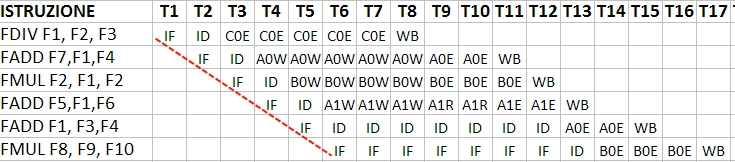
\includegraphics[width=\columnwidth]{img/tomasEs1}
\caption{Dinamica dell'esecuzione nel caso di 2 \textit{reservation station} per unità funzionale.}
\label{fig:tomasEs1}
\end{figure}
Indichiamo:
\begin{itemize}
\item con IF la fase di \textit{fetch};
\item con ID la fase di \textit{decode};
\item con le terne YXZ la \textit{reservation station} di indice X riservata all'operazione di ADD (Y = A), MUL (Y = B), DIV (Y = C), mentre siamo in attesa dell'operando (Z = W = WAIT), oppure quando l'operando è pronto ma non possiamo calcolare perché siamo privati dell'unità funzionale (Z = R = READY) o infine mentre stiamo effettuando la nostra operazione (Z = E = EXECUTE). Ad esempio: A0E = \textit{reservation station} 0 riservata alla ADD, stiamo calcolando la somma (E);
\item con WB la fase di \textit{write back}.
\end{itemize}

Una prima cosa che possiamo notare è che ogni istruzione entrante nella \textit{pipeline} deve anzitutto effettuare la \textit{fetch} (diagonale rossa). Ciò è sempre vero, qualsiasi sia lo stato delle alee o il numero delle istruzioni in gioco: non è però sempre detto che la \textit{fetch} duri un unico clock o che sia seguita immediatamente la fase di \textit{decode}. L'ultima ADD, infatti, è obbligata a stallare in ID in quanto non vi sono \textit{reservation station} libere (A0 è occupata e siamo in attesa di ricevere l'operando F1 dalla prima DIV per poter eseguire F1 + F4 => F7; anche A1 è occupata perché sta attendendo F1): se avessimo avuto tre RS per ogni unità funzionale (v. oltre) l'ultima ADD non avrebbe dovuto stallare in ID ma avrebbe potuto immediatamente procedere con una A2E. Notiamo inoltre che l'ultima istruzione (MUL) rimane in \textit{fetch} intanto che la ADD immediatamente precedente stalla in ID per carenza di RS (\textit{alea strutturale}).
Torniamo in cima: la DIV è la prima istruzione è può immediatamente partire, perciò la sua evoluzione temporale è ovvia (IF, ID, 5 cicli per effettuare l'operazione, WB). La prima istruzione, qualsiasi sia l'esercizio, può sempre andare immediatamente in EXECUTE, non dovendo attendere operandi da altre istruzioni.
La seconda, purtroppo, non può fare altrettanto: F1, infatti, deve prima essere aggiornato dall'istruzione precedente, eventualità che si verifica a seguito della fase di WB della DIV (in T8). Notiamo infatti che si ha A0W (attesa di operandi) da T4 fino a T8 e quindi A0E per i due cicli successivi. Attenzione: la fase di EXECUTE comincia sempre il ciclo successivo la WB dell'istruzione precedente che ha aggiornato l'operando!
Nel frattempo anche la MUL è costretta ad aspettare il WB della DIV (T8) per poter partire: l'evoluzione di tale MUL si snoda quindi in modo assolutamente analogo alla ADD precedente. Si noti che è possibile effettuare parallelamente una ADD, una MUL e una DIV (e infatti in T9 e T10 abbiamo due fasi E contemporanee), ma è assolutamente impossibile effettuare simultaneamente due operazioni dello stesso tipo: una buona verifica della bontà della soluzione è quindi quella di controllare che non vi siano mai più di una ADD o più di una MUL o più di una DIV contemporaneamente in esecuzione!
Dopo la MUL, ecco un'altra ADD: siamo salvi, abbiamo infatti occupato solo una delle due RS disponibili! In T6, quindi, possiamo scrivere A1W e metterci nuovamente in attesa dello stramaledetto F1 in uscita dalla DIV. Quel che non possiamo fare è invece eseguire la ADD in T9: già una ADD è infatti in esecuzione (A0E), quindi l'unica è riparare su A1R (READY: l'operando F1, richiesto, è pronto, ma non possiamo ancora eseguire a causa di \textit{alea strutturale}).
T10 è l'ultimo ciclo di clock in cui l'unità funzionale delle ADD è occupata: in T11, quindi, A1R può passare in A1E.
L'ultima ADD è costretta a stallare in ID, come già abbiamo sottolineato: ma non facciamoci ingannare! Quand'anche la \textit{reservation station} A0 si libera non possiamo fiondarci ad assegnare un identico \textit{tag} alla nostra nuova istruzione! Prima dobbiamo effettuare la "'vera'" ID (in T12, "'causata'" dal WB nel precedente T11) e quindi solo in in T13 possiamo scrivere A0E anche per la nostra ADD.
L'ultima MUL rimane invece in IF intanto che la ADD precedente stalla in ID; in T13 arriva il turno della MUL e infine si hanno tre cicli di esecuzione (B0E) prima dell'ultimo WB. \\

\begin{figure}[!h]
\centering
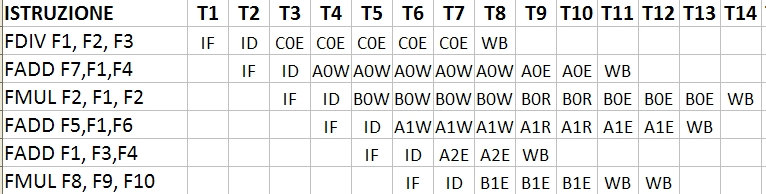
\includegraphics[width=\columnwidth]{img/tomasEs1b}
\caption{Dinamica dell'esecuzione nel caso di 3 \textit{reservation station} per unità funzionale.}
\label{fig:tomasEs1b}
\end{figure}

Se disponiamo di 3 RS (invece che 2) per unità funzionale, risparmiamo qualche \textit{clock} rispetto al caso precedente, in quanto possiamo evitare l'alea strutturale dell'ultima ADD. In figura \ref{fig:tomasEs1b} si mostra tale risultato: si noti che i clock totali sono 14 invece che 17, per uno \textit{speed-up} pari a 
\[
\dfrac{17}{14} = 1,214
\]
Il risparmio è dovuto principalmente alla velocizzazione delle ultime due istruzioni, come già anticipato: in particolare, l'ultima ADD può sfruttare un vuoto della relativa unità funzionale, la quale non è utilizzata dalle altre due analoghe istruzioni a causa della mancanza di F1 (che ci tocca sorbire fino a F8). 
Si noti infine che, in caso di più WB contemporanee, è necessario far progressivamente stallare quelle delle istruzioni successive alla prima, nonché all'unica, istruzione che può davvero eseguire il WB\footnote{Si veda tuttavia il paragrafo \ref{sec:casiParticolari} per maggiori chiarimenti.}. Nell'esempio, il \textit{clock} incriminato è T11: la ADD sta effettuando il WB e l'ultima MUL è costretta a ripeterlo in T12.

\section{Film delle variazioni dei registri}
\label{sec:filmRegistri}

\textsf{Si mostri il film delle variazioni dei registri F1 e F8 immaginando, per semplicità, che all'inizio si abbia $Fi=i$.}

\begin{figure}[!h]
\centering
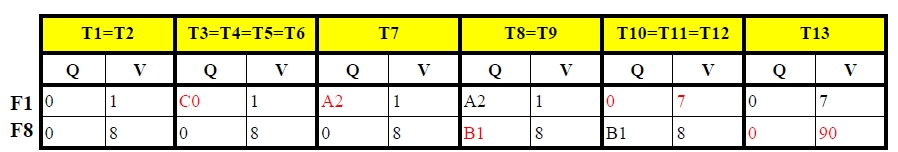
\includegraphics[width=\columnwidth]{img/tomasEs1c}
\caption{Film delle variazioni dei registri}
\label{fig:tomasEs1c}
\end{figure}

Mostrare il film dei registri significa illustrare l'evoluzione della coppia di valori Q e V per i registri richiesti. Il parametro V è il valore assunto da un determinato registro in un particolare momento, mentre Q può essere pari a 0 (se il valore V è quello attualmente valido) o pari all'identificatore della RS che "'restituirà'" tale risultato. Se Q è pari all'identificatore di una certa RS, allora significa che potremo porre Q = 0 e V pari al vero valore che il registro avrà in tale momento quando l'istruzione che ha prenotato quella \textit{reservation station} avrà effettuato il WB (o, più precisamente, il ciclo successivo). 
Esaminiamo la figura \ref{fig:tomasEs1c} e il registro F1: inizialmente la coppia (Q,V) sarà (0,1) in quanto il valore di partenza del registro F1 è (per ipotesi) 1 ed è un valore già disponibile e, per così dire, "'aggiornato'". Ogni volta che un'operazione prenota una \textit{reservation station} per il calcolo del valore di F1 dobbiamo impostare nuovamente il parametro Q: così ad esempio avviene in T3 (la DIV passa in C0E e quindi Q = C0) e in T7 (la ADD va in A2E e quindi Q = A2). Il valore V, in entrambi questi casi, non va toccato: esso va invece aggiornato nel ciclo successivo alla WB associata alla \textit{reservation station} corrispondente al valore Q. Nel nostro caso, Q = A2, quindi dobbiamo aggiornare V il ciclo successivo a quello in cui l'ultima ADD (quella che ha prenotato la \textit{reservation station} A2) ha effettuato il WB (cioè in T10, quando F1 diventa pari a 3 + 4 = 7).

Detto questo, il film di F8 diventa una banalità: la prima volta in cui un'istruzione bussa ad una RS per F8 avviene in T8, quando la MUL prenota la \textit{reservation station} B1: in T8 andremo quindi a scrivere Q = B1. Se nessun'altra istruzione vuole scrivere su B8 (e, per fare ciò, prenota una RS), dovremo aggiornare il valore V di F8 il ciclo successivo in cui la MUL avrà eseguito il WB. Quanto detto è effettivamente ciò avviene: in T12 la MUL effettua il WB e in T13 il valore del registro viene aggiornato.

\section{Film delle variazioni delle RS}
\label{sec:filmRS}

\textsf{Si mostri il film delle variazioni della RS B0 nel caso di 3 RS per unità funzionale, immaginando per
semplicità che all'inizio si abbia $Fi=i$.}\\

\begin{figure}[!h]
\centering
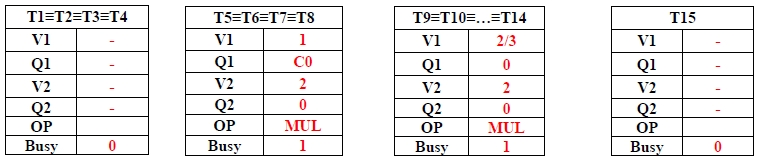
\includegraphics[width=\columnwidth]{img/tomasEs1d}
\caption{Film delle variazioni delle \textit{reservation station}}
\label{fig:tomasEs1d}
\end{figure}

La metodologia e l'approccio non è tanto diverso rispetto al caso precedente: in ogni RS sono presenti due coppie (Q,V), riservate ciascuna ad un operando dell'operazione che prenoterà la RS. I valori di Q e V all'interno della RS variano con le stesse modalità descritte nel paragrafo \ref{sec:filmRegistri}.
Nel nostro caso si chiede di disegnare il film della RS B0: la prima istruzione a prenotarla è la \{MUL F1, F2, F1\} quindi dovremo andare a scrivere le coppie (Q,V) di F2 e F1. F2 non è mai stato toccato quindi gli assegneremo il valore di \textit{default}, cioè 2, scrivendo la coppia (0,2); F1, invece, è il fastidiosissimo registro monopolizzato dall'altrettanto fastidiosa DIV, la quale ha prenotato la RS C0 in T3. La coppia (Q,V) sarà quindi (C0,1) e varierà in (0,2/3) il ciclo successivo al WB della DIV. La \textit{reservation station} B0 potrà quindi essere disimpegnata il ciclo successivo al WB dell'istruzione che l'ha prenotata (la MUL: WB in T14 e rilascio in T15).

\section{Miglioramento delle prestazioni: calcolo dello \textit{speed-up}}
\label{sec:viagra}

\textsf{Si calcoli lo \textit{speed up }di entrambe le soluzioni rispetto al caso di una sola unità funzionale capace di
eseguire le tre istruzioni e si commenti il risultato}.\\

Nel caso di una sola unità funzionale non in pipeline il numero di \textit{clock} necessari è dato dalla semplice somma della durata di tutte le istruzioni (da considerarsi come eseguite in maniera sequenziale). Nel nostro caso è data da: 
\begin{itemize}
\item 1 clock per la IF
\item 1 clock per la ID
\item 2 clock per ogni ADD (per un totale di 6)
\item 5 clock per ogni DIV (per un totale di 5)
\item 3 clock per ogni MUL (per un totale di 6)
\item 1 clock per il WB
\end{itemize}
Il totale restituisce 20 clock, risultato piuttosto modesto confrontato coi 17 e i 14 clock che si hanno nel caso di due e tre RS per ogni unità funzionale. L'incremento delle prestazioni dovuto all'inserimento delle RS può essere quantificato tramite il parametro \textit{speed-up} calcolabile semplicemente come rapporto fra i clock della caso più "'lento'" rispetto a quelli del caso più "'veloce'" (cioè con apportato il miglioramento in questione). \\
\textit{Speed up} con 2 RS: 
\[
\dfrac{20}{17}=1,176
\]
\textit{Speed up} con 3 RS:
\[
\dfrac{20}{14}=1,429
\]

\section{Casi e domande particolari}
\label{sec:casiParticolari}

\begin{itemize}
\item Nel caso di istruzioni che tentino di effettuare contemporaneamente un WB, abbiamo detto nel paragrafo \ref{sec:dinamicaTomasulo}, le istruzioni "'successive'" alla prima che riesce ad effettuare il WB dovranno ripetere tale fase per poterla effettivamente compiere. S'intende però che ha la precedenza chi, per prima, è andata in \textit{execute} e può accadere che un'istruzione dichiara diverse "'posizioni'" sotto un seconda istruzione sia in grado di effettuare il WB prima di quest'ultima. 
Ad esempio:
\begin{verbatim}
ADD   F18, F1, F22       IF  ID  ...  ...  A0W  A0E  ...  ...  WB   WB <- !!
...
...
MUL   F19, F3, F2        ... IF  ID   B0E  B0E  ...  ...  ...  WB  
\end{verbatim}
\item Se si chiede di provare a cambiare l'ordine delle istruzioni, e di verificare possibili aumenti prestazionali dovuti ad un conseguente risparmio di cicli di \textit{clock}, bisogna stare attenti a non farsi prendere dalla mano e verificare che il nuovo ordine non alteri il valore dei registri. Non è la stessa cosa fare $(1+2)\cdot 3$ piuttosto che $1 + (2\cdot 3)$!
\item Se si chiede di calcolare il minimo numero di cicli di \textit{clock}, qualunque sia il numero di RS, CRB e stadi di \textit{fetch} e \textit{decode} disponibili, basta effettuare il procedimento seguente: si calcola il massimo fra i seguenti prodotti
\[
\text{Numero di istruzioni di tipo X} \cdot \text{Clock impiegati per l'esecuzione dell'istruzione X}
\]
Quindi, se la ADD impiega 3 clock (4 ADD da effettuare), la MUL impiega 4 clock (2 MUL da effettuare), la DIV impiega 6 clock (3 DIV da effettuare), dovremo calcolare il massimo fra
\[
3\cdot 4 = 12  ~~~~~ 4\cdot 2 = 8  ~~~~~ 6\cdot 3 = 18 
\]
A questo risultato vanno sommati 2 clock (uno per ID e uno per IF) e tanti cicli di WB quante sono le istruzioni effettuate (il WB è obbligatorio e solo un ciclo dopo la sua messa in atto una nuova istruzione precedentemente in \textit{ready} o in \textit{waiting} può partire! Questo implica un'attesa di un clock per ogni istruzione).
\item Il numero di cicli di clock impiegato nell'elaborazione nel caso puramente sequenziale (non in \textit{pipeline}) è invece pari a 
\[
3 + \sum_i \left( \text{Numero istruzioni di tipo \textit{i}} \cdot \text{Clock per istruzione di tipo \textit{i}} \right)
\]
dove il 3 contiene le fasi di ID, IF e WB.
Prendendo in considerazione l'esempio del punto precedente abbiamo quindi
\[
3 + (12 + 8 + 3) = 26~ \text{ clock}
\]
Un calcolo analogo può essere trovato nel paragrafo \ref{sec:viagra}.
\item Con $k$ CRB fino a $k$ istruzioni possono effettuare contemporaneamente un WB "'valido'".

\end{itemize}
